\documentclass{ctexart}
\usepackage{graphicx}
\usepackage{amsmath}
\usepackage{amsthm}
\usepackage{amssymb}
\usepackage{fancyhdr}
\usepackage{ifthen}
\usepackage{syntonly}
\usepackage[colorlinks, CJKbookmarks=true, linkcolor=red]{hyperref}
\pagestyle{plain}
\usepackage[raggedright]{titlesec}
\newtheorem{性质}{性质}
\newtheorem{定理}{定理}
\newtheorem{推论}{推论}
\begin{document}
\title{作业}
\author{计算机科学与技术系52班 杨定澄 \and 学号:2015011274 \and E-mail:892431401@qq.com}
\date{}
\maketitle
\section{生成数据}
rand.py用于产生数据,运行得到的A1,B1,C1,A2,B2,C2的数据存在对应名字的.txt里。

现已生成好。
\section{KNN方法}
KNN.cpp实现了用KNN方法进行分类。

该算法复杂度为$O(KN^2)$,由于数据规模不小,为了提高效率我和造数据的python分开使用c++编写程序,后面同理。

手动实验了$K=3$到$9$的所有取值,可以看出针对该组数据,$K=9$时最优,A,B,C类的正确率分别为$97\%,83\%,98\%$,平均下来有$92.67\%$;$K=5$最劣,分别为$96\%,82\%,98\%$,平均下来$92\%$。

总之都在$92\%$以上。

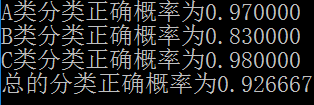
\includegraphics{1.png}

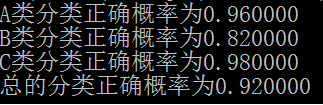
\includegraphics{2.png}


\section{线性分类机法}
linear.cpp实现的是线性分类机法。

我采用的方法是对于每一类做一次二类线性分类机,即对于$A$类,我把$B,C$全都看作是“不在$A$类”,然后最小化感知器准则函数。对于$B,C$类同理。

如此一来,得到了三个分类器,即三个感知器准则函数。对于某一个数据具体在哪一类,我采用的方法是分别计算三个感知器准则函数,哪个函数最大就在哪一类。

分类的效果如下图:

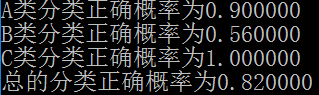
\includegraphics{3.png}

平均下来是$82\%$,可以看出对于$A$类,$C$类,效果都比较优,但是对于$B$类效果却比较差。

我们观察$A,B,C$服从的分布,发现$A$的均值集中在$(1,1,1)$,$B$的均值集中在$(3,3,3)$,$C$的均值集中在$(7,8,9)$。

直观的来看,可以感觉到$A$类所处位置大概在“三维情况下的左边”,$C$类大概在“三维情况下的右边”,$B$类正好在中间。

也就是说,对于$A,C$类,我们是能很轻松的分开的,比如我要分把$A$当一类$B,C$当一类分开,那么基本上就是在$A,B$间切一刀。$C$类同理。

但是$B$类并不容易做到,因为切在左边就把$C$分进去了,切在右边就把$A$分进去了,所以基本上分不开。

好在我们的算法是三种感知器函数取最大值,所以即使我在左边切一刀,$C$类也比较容易倾向于分进$C$类,$A$类同理,所以对于$A,C$类的分类影响不大,对于$B$类则大约一半的正确率。

这也就是线性分类机的局限之一了,因此,我们可以采用扩展的线性分类机的方法。

\section{扩展线性分类机(二类)}
我们不是直接对$(x,y,z)$做分类,而是进行投影映射。

linear1.cpp实现了扩展线性分类机,将三维空间中的一条直线映射成了一条抛物线。

$g(x)=a^Ty,y(x)=a_1+a_2x+a_3x^2$,在这里取得向量$a$是$9,6,1$。

这种方法有效避免了“不是$B$类”的区域多连通的情况。

分类结果如下

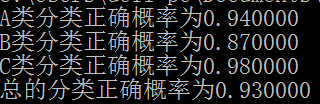
\includegraphics{4.png}

\end{document}
